\section{Introduction}

As communication devices and sensor infrastructures scale at a rapid
rate, it has now become possible to deploy large ad-hoc networks that
communicate in a limited fashion without a centralized control, and
carry out useful tasks (such as surveillance and threat detection)
even with limited coordination and control. This naturally leads us to
the consideration of {\em distributed} algorithms that use little or
no central control.

The lack of control is further exacerbated by the lack of complete
information about the environment in which the agents are located,
adding an extra layer of uncertainty to the problem. The paucity of
information can be modeled either by providing a probabilistic model
of the information which leads to {\em stochastic optimization}
models~\cite{bl97,rs06}, or by an adversarial model of information
revelation that leads to competitive analysis in the sense of {\em online
optimization}~\cite{be98,gkr10}. When the scenarios of uncertainty are neither quantifiable using randomness, nor adversarial, the framework of {\em robust optimization} models~\cite{BEN09,dgrs05} is also useful.

In this proposal, we develop a variety of models for studying the
fundamental tasks of establishing and maintaining connectivity and
control in complex networked systems, which capture three important features.

\begin{enumerate}
\item Limited
communication between agents (necessitating distributed algorithms),
\item Online revelation of information over time (including robust
and competitive frameworks), with the input selection ranging from the
worst-case adversarial to stochastic choice (leading respectively to online and stochastic optimization algorithms), and 
\item Permit the development of
rigorous approximation algorithms with a polynomial running time that
provide provably good solutions with worst-case performance guarantees. 
\end{enumerate}

These three aspects of our model directly address in order the three main
characteristics in this BRC topic detailed as follows.
\begin{enumerate}
\item Problems with ''a high degree of decentralization" and ''limited communication between system components",
\item ''Not all relevant information of the
environment is known a priori, and is revealed incrementally to individual system
components", and 
\item ''The techniques are capable of producing high-quality solutions in a reasonable amount of time" where ''solution quality is measured against optimality", and ''analysis of these measures is expected to be mathematically rigorous."
\end{enumerate}

\subsection{Summary of technical goals}
%\section{Models}
\label{sec:goals}

The main goal of this project is to develop a comprehensive theory of
{\bf \em distributed online approximation}\/ algorithms for hard network
optimization problems.
\iffalse (Repeats what is in the prev para)
This proposal encompasses several challenging
aspects of mission-critical networked systems: (a) there is
considerable uncertainty in the inputs and the network environment
under which the systems operate; (b) the inputs as well as the
underlying network may, in fact, be under adversarial control; (c) the
algorithms running these networked systems need to be
fully-distributed.
\fi
Our framework encompasses three dimensions - locality, uncertainty, and temporality,
with two complementary aspects to each dimension, see Figure \ref{fig:dimensions}.
This gives rise to eight different categories of problems.
The hardest problems are those that require decentralized distributed solutions when
faced with an adversary that adaptively reveals the input over time. Different
problems have different characteristics when investigated in the context of
different categories. 

\begin{figure}
\centering
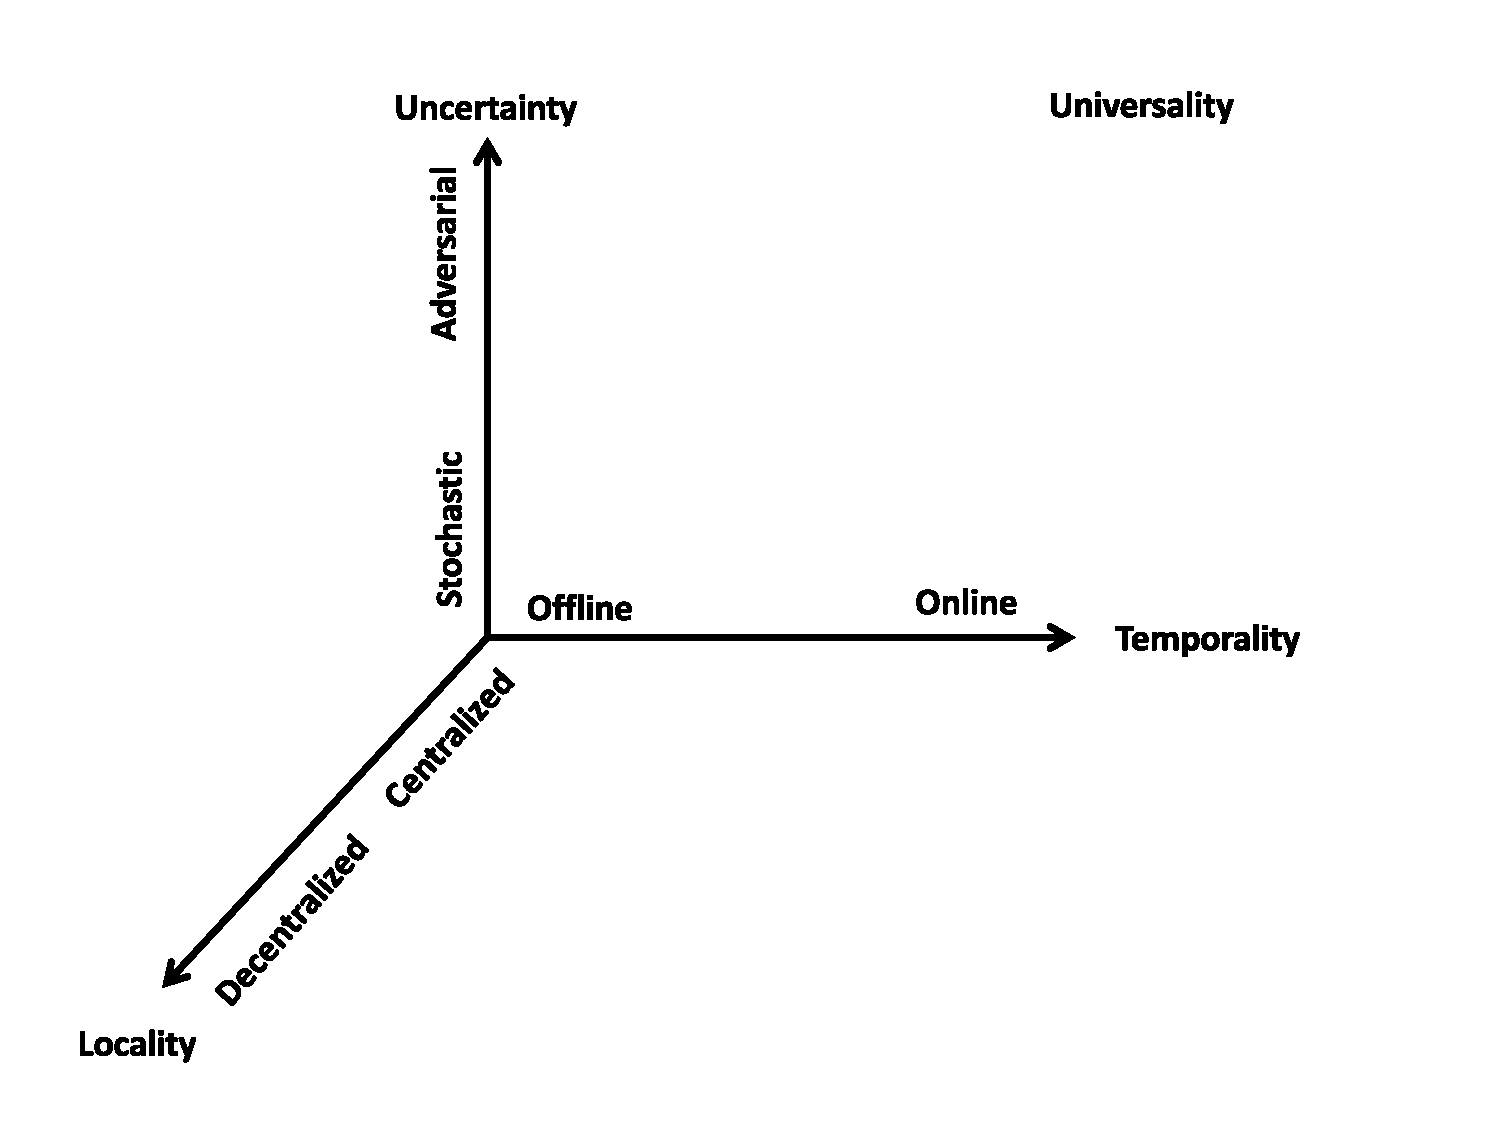
\includegraphics[width=4in]{dimensions-rev.ps}
\caption{Our framework for Distributed Online Optimization}
\label{fig:dimensions}
\end{figure}

In some fortunate circumstances, we can find solution
concepts that can handle multiple dimensions simultaneously as with the
(meta-)phenomenon of {\em universality} \cite{jia+lnrs:universal} that, for certain problems of central significance such as TSP, Steiner Tree and Set Cover, produces guaranteed solutions
(albeit,centralized)
in the face of adversarial revelation of the input; Indeed, universal algorithms
do not even exploit the adaptivity available to them and operate obliviously.
One of the hopes of this proposal is to extend the phenomenon of universality to
the distributed setting in addition to uncovering other similar (meta-)phenomena.


At a high level, the problems we plan to study in this project can be
divided into two categories: {\bf \em network design}\/ and {\bf \em
information flow}.
\medskip

\BfPara{Network Design} Network design concerns the construction of
overlay network structures that form the foundation for aggregation,
point-to-point routing, broadcast, multicast and other critical
network functions.  The deployment of mission-critical military
systems requires the ability to construct and maintain such
large-scale network structures that will enable secure and reliable
communication and operation in a highly dynamic and distributed
environment.  Research in network design has been at the forefront of
major advances in approximation algorithms~\cite{SWbook}.  We believe that
theoretical foundations of distributed online network design are
essential to achieve major advances in this area.  Within network
design, we will study the general problem of {\em survivable network
design}, with a focus on the important special case of {\em
aggregation trees}.

\begin{itemize}
\item
{\bf Survivable network design:} In the {\em survivable network design
  problem (SNDP)}, we are given a graph $G = (V,E)$ with edge-costs, and
edge-connectivity requirements $r_{ij} \in Z_{\ge 0}$ for every pair
of vertices $i, j \in V$, and need to find an (approximately)
minimum-cost network that provides the required connectivity.  This is
one of the most fundamental problems in network design that
generalizes several graph-theoretic optimization problems including
shortest paths, spanning and Steiner trees.  The edge-connectivity
requirements capture the need for increased reliability in
mission-critical systems; furthermore, the general statement of the
problem allows one to develop algorithmic paradigms that may have
broad applicability. {\em We propose the development of distributed online algorithms for the SNDP against strong adaptive adversaries.}

\item
{\bf Aggregation trees:} A special case of survivable network design
is the fundamental problem of constructing a tree that aggregates
information from important agents in a distributed network to a
central point (HQ). The agents are modeled as nodes in a graph, whose
edges capture the communication links between the agents.  Suppose the
primary task of the network is to detect and monitor specific targets
whose location the agents are unaware of a priori.  As the agents
explore their local terrain in detail they may become aware of the
presence of valuable targets. This converts such a node into a {\em
  terminal} node that must now communicate with the HQ node henceforth
called the {\em root}.  This problem is a variant of the classical
minimum Steiner tree problem.  Though Steiner tree and their variants
have been extensively studied, there are no distributed algorithms for
computing near-optimal Steiner trees in dynamic or uncertain
environments.  {\em We propose to build new distributed methods for constructing
near-optimal aggregation trees in stochastic and online environments, and design even more robust solutions in the form of universal approximations}.
\end{itemize}

\BfPara{Information Flow}
Information flow concerns the development of decentralized algorithms
that route higher-level application information over networks.  Within
information flow, we will study distributed algorithms for
constructing and maintaining routing tables, and gossip-based
information dissemination in highly dynamic networks.

\begin{itemize}
\item
{\bf Minimizing congestion in dynamic networks:} The capacity of links
in wireless (ad hoc and sensor) networks often changes due to fading
and multi-path effects.  Further, the mobility of the nodes themselves
leads to changes in the network topology.  A major challenge in such a
dynamic environment is to compute and maintain bottleneck-free routes
for information flow.  There are two main sources of difficulty:
first, the routes must satisfy certain degree constraints for
keeping routing information within manageable limits~\cite{xxx};
second, each node only has knowledge of the state of links to which
they are connected, while link capacities can be dynamically varying.
Given a traffic demand matrix over the set of nodes, our goal is to
devise a distributed algorithm that computes and maintains {\em
congestion minimizing degree-bounded flows}\/ between all
source-destination pairs.  The algorithm must be rapidly convergent
and must utilize minimal control information to avoid congesting the
links that must be conserved for data transport. {\em We propose to build distributed algorithms for congestion-minimizing multcommodity flows that also obey degree bounds.}

\item
{\bf Information dissemination in adversarially dynamic networks} The
dynamics of networks arising in military and critical infrastructure
settings are not only extensive, but can also be influenced by
external adversaries.  A natural model is that of an adversarial {\em
  time-evolving network}: in step $t$, the network $G_t = (V_t, E_t)$
is an arbitrary graph over the set $V_t$ of $n$ nodes, where the edge
sets $E_t$ are determined by an adversary.  We propose to develop
purely local lightweight algorithms for fundamental information
dissemination tasks in highly dynamic networks.  Our starting point
will be the basic {\em $k$-broadcast problem} in $k$ of the $n$ nodes
each have a message and would like to disseminate them to every node
in the network.  A fundamental open problem is the following: Can the
$k$-broadcast problem be solved on an dynamic, always-connected,
$n$-node network be solved in $O(n + k)$ steps? {\em We propose to design a distributed algorithm for this basic $k$-broadcast problem and develop fully distributed gossip-based algorithms for
consensus and aggregation.}


\end{itemize}

\subsection{Future Naval Relevance}

The problems presented in this proposal are of direct relevance to a number of Naval (and other military)
initiatives. The most notable example is JTRS \cite{feickert} - Joint Tactical Radio System.
JTRS is a Department of
Defense initiative to develop a family of revolutionary software-defined tactical radios
that will provide networked voice, data and video communications, as well as interoperability
across the joint battlespace. Originally conceived in 1997 it has expanded into an ongoing
family of programs for the development and delivery of tactical communications and networking
solutions for the Air Force, Army, Navy and Marines. Though portions of the JTRS program have
been scrapped or undergone transformation, nevertheless the research issues raised by some of
its subinitiatives continue to be of significance today.
The Airborne, Maritime, Fixed Station (AMF) subinitiative of the JTRS project is of particular
relevance.  It is concerned with the design, development, integration, testing and delivery of
advanced communication systems to modernize current radio systems with next-generation
Software Defined Radio technology. The properties of reliable network-centric capability and legacy
compatibility are to provide joint interoperability and secure information flow for
military platforms such as aircraft, submarines, surface ships and DoD installations.
The problems of {\em network design} and {\em information flow} are directly motivated by
applications to the AMF JTRS program.

There is immense ongoing interest in the development of an
IP-based Air-and-Surface borne Network based on mobile ad hoc
networking concepts. Such a network may consist of
disparate mobile airborne and sea-based platforms; will provide reliable ad
hoc interconnectivity to terrestrial and airborne nodes; and
will be applicable to net-centric military communications. A
wireless network that includes an airborne component is
architecturally reminiscent of conventional wireless
telecommunications networks. Relatively quasi-stable
airborne platforms, equipped with directional data links, could
form a high capacity backbone core akin to the back-haul in
telecommunications networks. This directional backbone core
would serve as a reliable data transport infrastructure for
highly dynamic terrestrial and airborne platforms at the
network edge, which are typically equipped with lower
capacity omni-directional radios. The latter are akin to end
users in conventional telecommunications networks.
As in any mobile network, the performance of such a network
depends to a great extent on the prevailing network topology.
The network topology determines the availability and the
characteristics of the data path between any two nodes of the
network. These characteristics directly dictate the performance
of data transmission, such as throughput and delay, between
the nodes. For a network of fixed nodes the topology is
essentially static. It is determined by deployed physical
connections between nodes. For a network with mobile nodes
the topology is dynamic with several topology choices
possible. The design problems of {\em survivable networks}
and {\em aggregation trees}  are motivated by the
need for active topology management and optimization in
these Air-and-Surface borne networks with
the aim to improve overall communication and decision-making performance.

In this proposal, we are interested not just in the management and
optimization of the topology but also the sharing and routing of
relevant information in a timely manner so as to satisfy mission-critical
needs. The movement of information on the network core is a challenging
proposition due, in particular, to the following factors: (1) The
nodes have a limited number of  directional links (and this
number may be different for different nodes), (2) The links
may have different and time-varying data rates (for instance, due to differences
in received Signal to Interference and Noise Ratio (SINR)),
(3) The nodes may be moving in space causing changes in underlying topology;
with incoming and outgoing links of different radio
types, such compatibilities introducing communication constraints over and above
range restrictions, and (4) There may be important information that needs
to get from one part of the network to the other at the same time as
jamming or eavesdropping adversaries are rendreing certain links inoperational.
Motivated by these issues we study the problems of {\em congestion
minimization} and {\em information dissemination} in dynamic networks.

\subsection{PI Information}
Prof. R. Ravi works in the intersection of Operations Research and
Computer Science and has pioneered work in various network
optimization problems such as the Buy-at-Bulk Network Design problem
with economies of scale, the Group Steiner Tree problem that combines
the Set Covering and Steiner Tree problems, and in designing provably
near-optimal approximation algorithms with performance guarantees for
problems in stochastic and robust combinatorial optimization. He has
also advanced the development of tools for the design of approximation
algorithms for network optimization such as the primal-dual method,
dependent randomized rounding, Lagrangean relaxations and iterative
methods.

Co-PI Rajaraman's research expertise covers distributed computing
theory, approximation algorithms, network optimization, and
algorithmic game theory.  His work on distributed hash tables is
widely-cited and has been implemented in several peer-to-peer network
systems.  Co-PI Sundaram's research expertise covers networks,
algorithms, complexity theory and combinatorics.  Before joining
academics, he was Director of Engineering at Akamai Technologies,
where he established the mapping group for the world's leading content
delivery network, which is responsible for directing browser requests
(over 10 billion a day) to the optimal Akamai server.

The PIs have a strong history of collaboration.  PI Ravi and co-PI
Sundaram were co-authors on a widely cited foundational paper on
bicriteria approximations in network design.  Co-PIs Rajaraman and
Sundaram were co-authors on a ICDCS 2006 paper on Internet capacity
that won the best paper award.  With deep synergistic expertise in
optimization theory, online and approximation algorithms, and
distributed computing, the team is uniquely positioned to address the
basic research challenges of this call.

